    %\begin{figure}
    %    \centering
    %    \includegraphics[width=0.5\textwidth]{DSNU fingerprint.png}
    %    \caption{DSNU fingerprint extraction}
    %    \label{fig:my_label}
    %\end{figure}.
\section{INTRODUCTION}
This article summarizing three notations covered in Formal specification study. And the start from section 4 the system designed in assignment 1 and assignment 2 will be explained. Furthermore, design in assignment2 will be extend with CSP to describe the operations between each class. 


\section{Three Notations}
\subsection{Z notation}
A specification of a system should aid understanding of that system, assisting development and maintenance of the system. Specifications need express only abstract properties, unlike implementations such as detailed algorithms, physical circuits, etc. Specifications may be loose, allowing refinement to many different implementations. Such abstract and loose specifications can be written in Z.
A specification written in Z models the specified system: it names the components of the system and expresses the constraints between those components. The meaning of a Z specification, its semantics is defined as the set of interpretations (values for the named components) that are consistent with the constraints.
Z uses mathematical notation, hence specifications written in Z are said to be formal: the meaning is captured by the form of the mathematics used, independent of the names chosen. This formal basis enables mathematical reasoning, and hence proofs that desired properties are consequences of the specification. The soundness of inference rules used in such reasoning should be proven relative to the semantics of the Z notation.\cite{Z}
\subsection{Object Constrain Language(OCL)}
OCL is a formal language used to describe expressions on UML models. On top of Z notations, OCL provide restriction on model or class. So the definition of each object could be modeled more clear. These expressions typically specify invariant conditions that must hold for the system being modeled or queries over objects described in a model.
Initially, OCL was only used as a constraint language for UML but quickly expanded its scope and now OCL has become a key component of any model-driven engineering technique as the default language for expressing all kinds of model query, manipulation and specification requirements. OCL expressions can be used to specify operations / actions that, when executed, do alter the state of the system. UML modelers can use OCL to specify application-specific constraints in their models. UML modelers can also use OCL to specify queries on the UML model, which are completely programming language independent.\cite{OCL}
\subsection{Communicating Sequential Processes (CSP) notation}
CSP was highly influential in the design of programming language and also influenced the design of programming languages such as Go. Communicating Sequential Processes, or CSP, is a language for describing patterns of interaction. It is supported by an elegant, mathematical theory, a set of proof tools, and an extensive literature. The book Communicating Sequential Processes was first published in 1985 by Prentice Hall International (who have kindly released the copyright); it is an excellent introduction to the language, and also to the mathematical theory.\cite{Barnes:2010:CPO:1713254.1713265}
\section{System Modeling}
In following sections, models designed through course with Z notation, OCL and CSP will be explained. System modeled using Z notation in Assignment 1 and Petrol System designed in Assignment 2 will be introduced. And the interactions in Petrol System will be further developed, using CSP notation.
\section{Electronic Key System}
In this design, a key system model has been presented. This model includes three main states: KEY, ROOM and EKS. KEY contains only one information,KeyID.ROOM contains ID and Status of either locked or unlocked. EKS is the core of this system, it maintains management of rooms and keys. An important property Pairs is used to store relationship between ROOM and Key. So, domain of Pairs would fall in to Rooms set and ranges of Pairs is inside set Keys. 

In EKS initiation, all Rooms, Keys and Pairs are set to empty and constant SIZE\char`_K, SIZE\char`_R` is initialized. Use those too constant, as restriction factor of fixed size set of Rooms and Keys. In schema operation like AddKey, AddRoom, if the size of set Keys, Rooms has achieved it maximum, then the addition could not be operated. 

\textit{AddRoom} and \textit{AddKey} is designed in similar manner. The operation check input candidate with exists ROOM/KEY, add candidates to key system if no redundancy has been found. 
Relative to addition, \textit{RemoveKey} and \textit{RemoveRoom}, will check is the key/room is one of the elements inside Keys or Rooms. Additionally, any removal of KEY/ROOM will remove its relationship from Pairs. Imaging in real environment, if a key is removed from key system, it shall not able to open any room. Similarly, if a room is removed from the system, no any key will unlock the room. 

\textit{RescindRoomAccess} removes relationship of given KEY and ROOM from Pairs
\textit{GrandRoomAccess} add a relationship of given KEY and ROOM to the Pairs. Additionally, the Key will only in relationship with the Room. In another words, if a key grands access of room this key can only unlocked this specific room and verse versa. 

\textit{GrandRoomAccessMulti}, is the extra bit consideration from GrandRoomAccess. In real scenario, a hotel manager always has access to the room. In design term, a KEY shall be able to unlock multiple ROOM if use this operation. This operation only appends new ROOM-KEY relationship to the Pairs, which will not change the previous relationships.

\textit{OpenRoom}, \textit{LockRoom}, first check if the given Key is in Key system. Then, is the Room in the system. Also, is the relationship of given key and room being subset of Pairs. If all above have pass the check, alter the status of room. 

\section{The Shunting Game}
This game is designed with following schema and operations. 
Special consideration has been taken in terms of \begin{itemize}
    \item Pieces could only move to a location which belong to Board
    \item How white piece shall move while black piece took it position
\end{itemize}
First of all, a Board is using to describe the playground. 
Shunting schema includes information regarding to position of black and white pieces and the score of game. 
\textit{ShuntingINIT}: initialized pieces\char`' positions and game score.
Function \textit{next} has described what can be defined as the relationship between two board position. If two position next to each other, it shall have following relationship:
\begin{align*}
x_1 &= y_1  &   x_2 &= y_2 + \pm1  \\
x_2 &= y_2  &   x_1 &= y_1+ \pm1
\end{align*}
\textit{Beyond}: returns the white piece position after being pushed by a black piece.
Therefore, we have three elements,
\begin{itemize}
    \item 	black - location of black piece
    \item 	white - the location of white piece before been pushed 
    \item 	result - the final location of white piece after pushed 
\end{itemize}

On x-y coordinate system, those three elements shall have the same value on x or y coordinate. According to the position of three element. Either x-coordinate or y-coordinate of those elements will shall a same value, because the push activity results the black piece, white piece and the pushed location on a same line. Finally, the white piece will be pushed forward for 1 unite. Therefore, use either (second white to second black) or (first white to first black) to address the change with \pm sign. 

\textit{Move}: this a operation used to move black piece around while A target position aka \textit{posn} is given. 
Consideration of relevant details are covered as following:
\begin{enumerate}
    \item 	Is the target position on Board, if it is outside the range of Board, no piece shall be moved. 
    \item 	If the black piece is moving towards a direction with two white pieces together on its path. And one of the white pieces is close to black piece. Then the move cannot be operated. 
    \item 	After every move, score one. 
    \item 	If the given target position is an empty space on Board, and it is next to the current position of black piece. Then move black piece to this position. 
\end{enumerate}

\section{OCL specified Petrol System}
\subsection{Introduction of Petrol System}
In this assignment, a petrol system has been modeled with detail restrictions. 
A petrol supply system can be informally described as follows. A petrol company owns a number of petrol stations. Each petrol station consists of a number of petrol pumps. Each pump can be reset by a supervisor, after which it can pump out petrol from a common store, recording at each stage the volume and cost of petrol pumped so far. When pumping is finished, the total cost is recorded by the supervisor and subsequently paid by the customer. Each pump in a petrol station sells petrol at the same price, although this price may vary between stations. The common store can be re-stocked by the petrol company at any time. The company supplies petrol at the same cost to each station. Records are kept of the total volume of petrol supplied to each station, as well as the outstanding amount owed by each station. The amount owed to the company by the station is paid when requested by the company.\cite{li2013object}
\begin{center}
    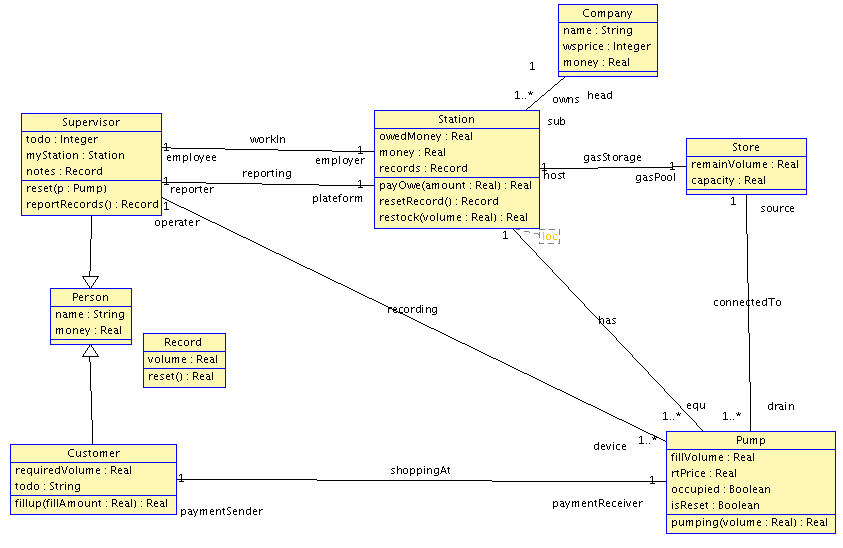
\includegraphics[angle=0,width=1\linewidth]{classDiag.png}
    \subsection{Design of Petrol System}
    \caption{Class Diagram}
    \label{fig:my_label}
\end{center}
\texit{Company} class is the source of petrol. In this petrol system, company provide petrol to each station and company can also collect the bill anytime. In the design, company will have \textit{money} attribute to indicate the total amount of money received from stations. While collect bill from stations, the variable money get increased. 

\textbf{Station} is an important class in this system due to the complex level. A station is connect to Store, which store fuel from company. A station also owns at least two pumps, pump will serve customer with fuel and bring a result of charges for each transaction.

\textbf{Pump} Special design has been considered for this class. Pump class provide function of pumping fuel for customer. It also has an attribute - retail price for the fuel. Put retail price in pump class will create potential possibility to extend the model for variate retail price at each pump. Of course, following the requirment, the invariant of \textit{samePriceAtPump} avoid the diversity. 

\textit{samePriceAtPump} ensures same petrol price at a station by add up all rtPrice from pumps in a station, and divide by number of pumps. While each rtPrice at pump is equivalent, the invariant will return true.

\textit{Pumping} is an operation of a \textbf{Pump}, it checks prerequisites of both user and pump before it performs the action of providing gas. And after the pumping it will be idle and in a status of waiting for supervisor.

\textit{Record} helps logging the transaction system wide.\textbf{ Station} keeps an instance of \textit{Record} so the amount of money a Station need pays to the Company is clear. \textit{Record} also exists as an attribute in \textit{Supervisor}. By doing this, Supervisors can record the transaction at pump and report to the Station later on. The design diversity here could be either customer gives money to superviosr and superviosr collect all the money from transactions at each pump and transfer this amount of money to Staion once a while. 

\textit{reportRecords} is the operation in  \textbf{Supervisor}, the precondition make sure a supervisor have non-zero content to report. And the precondition also checks whether the supervisor is currently employed by particular station he/she report to. It also ensure the supervisor have logged all pumps before she reports. For example, if someone is pumping fuel at a pump, the supervisor shall wait until he finishes and collect the transaction before the superviosr report his record to station. 

\textit{Customer} and \textit{Supervisor} are both \textit{People}, in this system they are inherent from People class and have different interaction relationship with pump. Where customer get fuel and pay for the transaction at Pump, supervisor collects the transaction.

\section{CSP of Petrol System internal interactions}
In this section, the petrol system design from OCL model will be further developed. As the specialization of CSP, the design will be focus on the internal interactions of operation between Pump, Station, Store and Customer, Supervisor,etc.
\subsection{Operation design}
Design with Communicating Sequential Processes here is essentially focus on interactions of operation. 
\subsubsection{Timeout at pump}
While a pump has not received any instructions for 2 minutes, it shall return to it\char's initial status.
\begin{lstlisting}[captionpos=b, %caption=Fuel Transfer,
   ,basicstyle=\ttfamily]
-- Timeout at pump
(Customer->Paid)[>{60}
    (shutdown->STOP)
Wait t; Pump = STOP [> {t} Pump
\end{lstlisting}
\subsubsection{Money Transfer}
In this piece of design, money paid by customer are directly received by supervisor, and only after that the fuel can be pumped. 
\begin{lstlisting}[captionpos=b, %caption=Fuel Transfer,
   ,basicstyle=\ttfamily]
-- Money transfer
datatype Paid = ten | twenty | thirty
channel station,supervisor, customer, money:Paid
SEND = customer?m ->supervisor!m ->store->SEND
RECI = supervisor?m ->station!m ->RECI
SYSTEM = (SEND[|{|supervisor,money|}|]RECI)
         \{|supervisor,money|}

\end{lstlisting}
\subsubsection{Fuel Transfer}
While a customer request fuel at pump. The fuel will sent from store to pump and then to the customer. 
\begin{lstlisting}[captionpos=b, %caption=Fuel Transfer,
   ,basicstyle=\ttfamily]
-- modelling fuel transfer
datatype FUEL = ultimate | premium | diesel 
channel store, customer, pump:FUEL
channel record

SEND = store?x ->pump!x ->record->SEND
RECI = pump?x ->customer!x ->record ->RECI
SYSTEM = (SEND[|{|pump,record|}|]RECI)
         \{|pump,record|}
GEN = store!ultimate ->GEN[]store!premium 
        ->GEN[]store!diesel->GEN
MAIN=SYSTEM [|{| store |}|] GEN
\end{lstlisting}
\section{Conclusion}
All three notation are useful in software development. Where Z notation focus on description of the model, OCL adds constrain condition to deisgn model.And CSP could address the interactions between class. And during the research there are some problems of CSP are spotted.Explicit naming of communicating. If a value passed from process A to process B have different data type than the assigned value, the both processes will crash. Also if the output processes refers to a terminate process, it is going terminate too. No proof method. A serious problem of CSP is that it does not have any assist in development and verification of correct program. Even though, those three notation are still helpful in software development. 

